\section{Signal preprocessing}
The vibration signals in a factory environment are inherently full of disturbances from adjacent equipment or irregular movement during object manipulation in the surrondings. In addition, accelerometers suffer from systematic measurement errors in the form of zero-g offset and bias that originates from a constant force of gravity. These unavoidable distortions are suppressible to some extent with digital filters. In the preprocessing stage we consider detrending, noise reduction with adaptive filters, and time synchronous averaging to supress interference among components.

\subsection{Detrending}
The oscillatory motion should be centered around the zero level for further manipulation. The constant offset is eliminated simply by subtracting the overall average from the signal. Moreover high pass DC blocker infinite impulse response (IIR) filter of 1st order can adjust to shifts of the mean value (Equation~\ref{equ:iir-dc-blocker}). The transition band depends upon the choice of corner frequency $f_{3dB}$ (Fig.~\ref{fig:dc-blocker}).

\begin{equation} \label{equ:iir-dc-blocker}
y_k = (1 - \frac{\omega}{2}) \cdot (x_k  -  x_{k - 1}) + (1 - \omega) \cdot y_{k - 1}; \quad \omega = 2\pi \cdot \frac{f_{3dB}}{f_s}
\end{equation}

A steeper 3~dB attenuation band can be achieved by increasing the order of the filter. Then the cutoff frequency should be such that filter coefficients are fractional numbers to counteract rounding errors~\cite{tittelbach-helmrich_digital_2021}.

\begin{figure}[h]
	\centering
	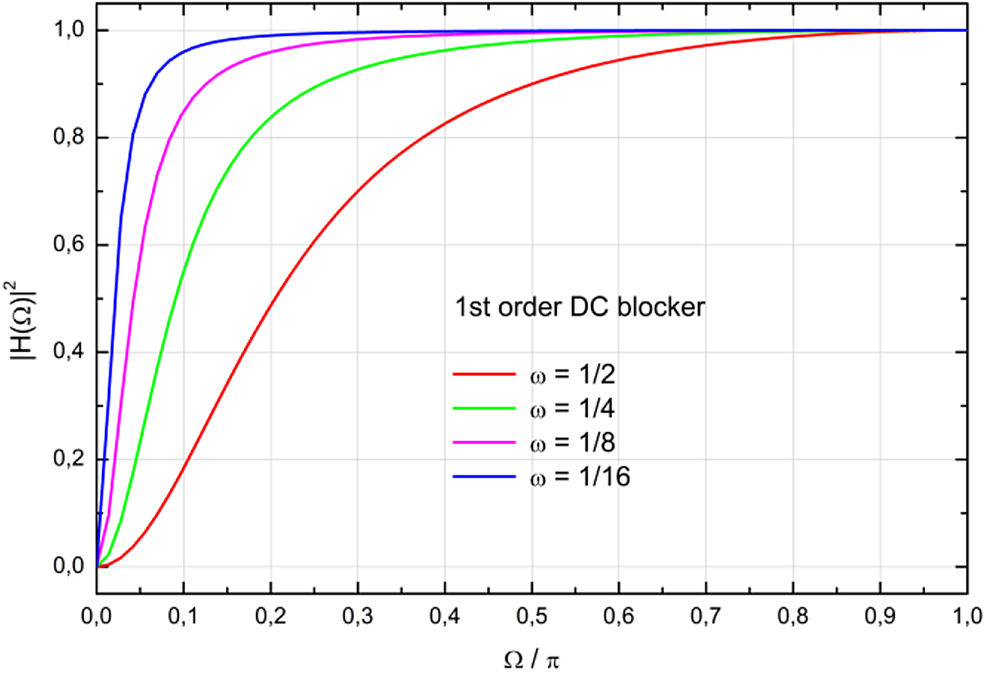
\includegraphics[width=0.7\textwidth]{assets/iir-1-dc-blocker-band.jpg}
	\caption{Transfer function of 1st order DC blocker filters ~\cite{tittelbach-helmrich_digital_2021}}
	\label{fig:dc-blocker}
\end{figure}

The finite impulse response (FIR) filter is not recommended for DC component removal because of the undesirable ripple effect with the small number of taps. Cascaded-integrator-comb (CIC) filters are proposed as an alternative instead~\cite{lyons_understanding_2011}.

\subsection{Adaptive noise cancellation}
Adaptive noise cancellation (ANC) involves an adaptive filter that self-adjusts coefficients through an update algorithm in response to the reference noise signal.  The objective of this filter is to minimize the cost function of mean square error (MSE) in error signal $e_k$ between signal contaminated with additive Gaussian noise $d_k$ and filter output $y_k$. Additive noise $n_k$ is assumed to be correlated with noise signal $\mathbf{X_k}$~\cite{diniz_adaptive_2020}.

Wiener-Hopf equations solve the optimal gradient of MSE function and FIR filter coefficient vector $\mathbf{W_k}$.  The least mean squares (LMS) algorithm recursively approximates this analytical solution with the method of steepest descent (Equation~\ref{equ:lms-adaptive-filter})~\cite{diniz_adaptive_2020}. The multiple parameters are to be considered in the evaluation of filter performance: convergence rate, estimated error, and signal-to-noise ratio (SNR).

\begin{ceqn}\begin{align} \label{equ:lms-adaptive-filter}
\mathbf{W}_{k+1} = \mathbf{W}_{k} + 2 \mu \mathbf{X}_{k}  e_k
\end{align}\end{ceqn}

The convergence stability is affected by step size $\mu$ which is bounded from above with the inverse of the maximal eigenvalue of input covariance matrix $\lambda_{max}$. The normalized least mean squares (NLMS) can handle input of varying scales  (Equation~\ref{equ:nlms-adaptive-filter}).

\begin{ceqn}\begin{align} \label{equ:nlms-adaptive-filter}
\mathbf{W}_{k+1} = \mathbf{W}_{k} + \frac{\mu}{\lVert\mathbf{X}_{k}\rVert^2} \mathbf{X}_{k}  e_k
\end{align}\end{ceqn}

\begin{figure}[h]
	\centering
	
\includegraphics[width=0.8\textwidth]{assets/adaptive-filter.png}
	\caption{Adaptive noise cancellation filter diagram}
	\label{fig:adaptive-filter}
\end{figure}
\bigbreak

\subsection{Time synchronous averaging}
Time synchronous averaging is dimished the impact of sources unrelated to the harmonics of the rotational frequency in the vibrations. Time-domain waveform is averaged over $N$ points and aligned to synchronization pulse with period $T$ (Equation~ref{equ:tsa-average}). This technique has been successfully applied to the gearbox and bearing fault diagnosis~\cite{davies_handbook_2012,nandi_condition_2019}
\begin{ceqn}\begin{align}
x_{TSA} = \frac{1}{N} \sum_{n = 0}^{N - 1}{x(t + nT)}
\label{equ:tsa-average}
\end{align}\end{ceqn}

\section{Feature engineering}
Before the raw observations of the machine condition are input into a machine learning model, the descriptive and summarizing numerical attributes are calculated. The informative features are selected from the provided set to determine a diagnosis.

Among the main advantages of add-in extraction effort, as opposed to processing samples unmodified, is to gain better classification precision and reduce computational burden downstream through dimensionality reduction techniques. Predictive maintenance has ideal prerequisites for the application of feature engineering because the signal characteristics are pseudo-stationary, and the trend monitoring variables are established out of extensive domain expertise in mechanics.

The steps to undertake in the transformation of source data streams to a knowledge of machine status begins with
preprocessing that continues to feature extraction, then feature selection and the ultimate result is dependent on the model.

\subsection{Feature extraction}
% Feature Engineering for Machine Learning
\cite{zheng_feature_2018}
% Feature Engineering and Selection: A Practical Approach for Predictive Models
\cite{johnson_feature_2019}

% A Novel Online Machine Learning Approach for Real-Time Condition Monitoring of Rotating Machines
% - list of features
\cite{mostafavi_novel_2021}

% A New Statistical Features Based Approach for Bearing Fault Diagnosis Using Vibration Signals
% - knn with manhalobis distance
% - select features manually as oposed to CNN and RNN
\cite{altaf_new_2022}
$$X_{rms} = \sqrt{\frac{1}{N} \sum_{i=1}^{N}{x_i^2}}$$  % rms
$$X_{cf} = \frac{\max(|x_i|)}{X_{rms}}$$  % crest factor

$$ $$% standard deviation
$$X_{kv} = \frac{1}{N}  \sum_{i=1}^{N}{\frac{x_i - \bar{x}}{\sigma}} $$ % kurtosis


% Fault Detection of Bearing: An Unsupervised Machine Learning Approach Exploiting Feature Extraction and Dimensionality Reduction
% - Time domain: mean, standard deviation, rms (root mean square), peak value, peak-topeak value, shape indicator, skewness, kurtosis, crest factor, clearance indicator, etc. (ii) Frequency domain: mean frequency, central frequency, energy in frequency bands, etc. (iii) Time-frequency domain: entropy are usually extracted by Wavelet Transform, Wavelet Packet Transform, and empirical model decomposition.
\cite{brito_fault_2021}

FFT - Short Time Fourier Transform with Hamming window and Welch averaging
	% \cite{oulmane_automatic_2015}


% A large setof audio features for sound description
\cite{peeters_large_2004}
% Research on online intelligent monitoring system of band saw blade wear status based on multi‑feature fusion of acoustic emission signals
\cite{zhuo_research_2022}
% Early Detection of Imbalance in Load and Machine In Front Load Washing Machines by Monitoring Drum Movement
\cite{mohammadi_early_2020}
% A Data Mining based Approach for Electric Motor Anomaly Detection Applied on Vibration Data
\cite{egaji_data_2020}
% Condition Monitoring with Vibration Signals
\cite{nandi_condition_2019}

% Vibration Analysis for IoT Enabled Predictive Maintenance
\cite{jung_vibration_2017}

\paragraph{Statistical measures}
\begin{itemize}
\item Standard Deviation
\item Max. amplitude
\item RMS amplitude
\item Skewness
\item Kurtosis \\
---
\item Spectral centroid
\item RMS frequency
\item Root variance frequency
\item Spectral kurtosis / Fast kurtogram
\item Harmonics (peaks)
	% Multi-Scale Peak and Trough Detection Optimised for Periodic and Quasi-Periodic Neuroscience Data
	\cite{bishop_multi-scale_2018}
	% Non-Parametric Local Maxima and Minima Finder with Filtering Techniques for Bioprocess
	\cite{adikaram_non-parametric_2016}
	% Identification of harmonics and sidebands in a finite set of spectral components
	\cite{gerber_identification_2013}
	% Evaluation of Threshold-Based Algorithms for Detection of Spectral Peaks in Audio
	\cite{nunes_evaluation_2007}
\item Spectral Envelope
\item Harmonic spectral deviation \\
---
\item Energy
\item Spectral negentropy
	% Spectral negentropy and kurtogram performance comparison for bearing fault diagnosis
	\cite{avoci_spectral_2020}
\item TKEO - Teager-Kaiser energy operator
	%Application of Teager–Kaiser Energy Operator in the Early Fault Diagnosis of Rolling Bearings
	\cite{shi_application_2022}
\end{itemize}

\paragraph{Wavelet signal decompositions}

\begin{itemize}
\item CWT-SST - Synchrosqueezing Wavelet Transform
	% The fast continuous wavelet transformation (fCWT) for real-time, high-quality, noise-resistant time–frequency analysis
	\cite{arts_fast_2022}
	% A Concentrated Time–Frequency Analysis Tool for Bearing Fault Diagnosis
	\cite{yu_concentrated_2020}
	% Applications of the synchrosqueezing transform in seismic time-frequency analysis
	\cite{herrera_applications_2014}

\item WPD - Wavelet Packet Decomposition  - to approximation and detail coef. (Fejer-Korovkin wavelet)
	% Wavelet Packet Feature Extraction for Vibration Monitoring
	\cite{yen_wavelet_2000}
	% A wavelet approach to dimension reduction and classification of hyperspectral data
	\cite{wickmann_wavelet_2007}
	% The MFBD: a novel weak features extraction method for rotating machinery
	\cite{song_mfbd_2021}

\item EWT - Empirical Wavelet Transform - (Meyer wavelet)
	% Empirical Wavelet Transform - Gilles
	% On the computational complexity of the empirical mode decomposition algorithm
	\cite{wang_computational_2014}
	% Novel self-adaptive vibration signal analysis: Concealed component decomposition and its application in bearing fault diagnosis
	\cite{tiwari_novel_2021}
	% The MFBD: a novel weak features extraction method for rotating machinery
	\cite{song_mfbd_2021}
	% Fault Feature Extraction and Enhancement of Rolling Element Bearings Based on Maximum Correlated Kurtosis Deconvolution and Improved Empirical Wavelet Transform
	\cite{li_fault_2019}
	% An Improved Empirical Wavelet Transform for Noisy and Non-Stationary Signal Processing
	\cite{zhuang_improved_2020}
	% Time and frequency domain scanning fault diagnosis method based on spectral negentropy and its application
	\cite{yonggang_time_2020}
	% An Adaptive Spectrum Segmentation Method to Optimize Empirical Wavelet Transform for Rolling Bearings Fault Diagnosis
	\cite{xu_adaptive_2019}
	% Improved empirical wavelet transform (EWT) and its application in non‑stationary vibration signal of transformer
	\cite{ni_improved_2022}
\end{itemize}


\subsection{Feature transformation}
\cite{zheng_feature_2018}
\begin{itemize}
\item Normalization (min-max, standardize)
\item Log transformation (Box-Cox Transform) to normal distribution
\item Principal Component Analysis (PCA)  % \cite{brito_fault_2021}
\end{itemize}

\subsection{Feature selection}
Subset generation % p.193
Subset evaluation
Stopping criteria
Validation

\cite{nandi_condition_2019} % p.192
Filter method - SelectKBest  in evaluation phase
\begin{itemize}
\item Variance Threshold
\item Pearson correlation
\item ANOVA F-value
\item Mutal information
\item Fisher score
\item Spectral feature selection algorithm (SPEC)
\end{itemize}
